
%\definecolor{lightRed}{RGB}{255,130,130}
\definecolor{lightRed}{RGB}{255,115,115}

%%%%%%%%%%

\begin{frame}{\vskip -0.2cm \large The Breiman-Friedman-Olshen-Stone CART Algorithm}

\small

\begin{multicols}{2}

	\begin{flushright}
	\begin{minipage}{4.5cm}
	\vskip -0.4cm
	{\color{white}AAA}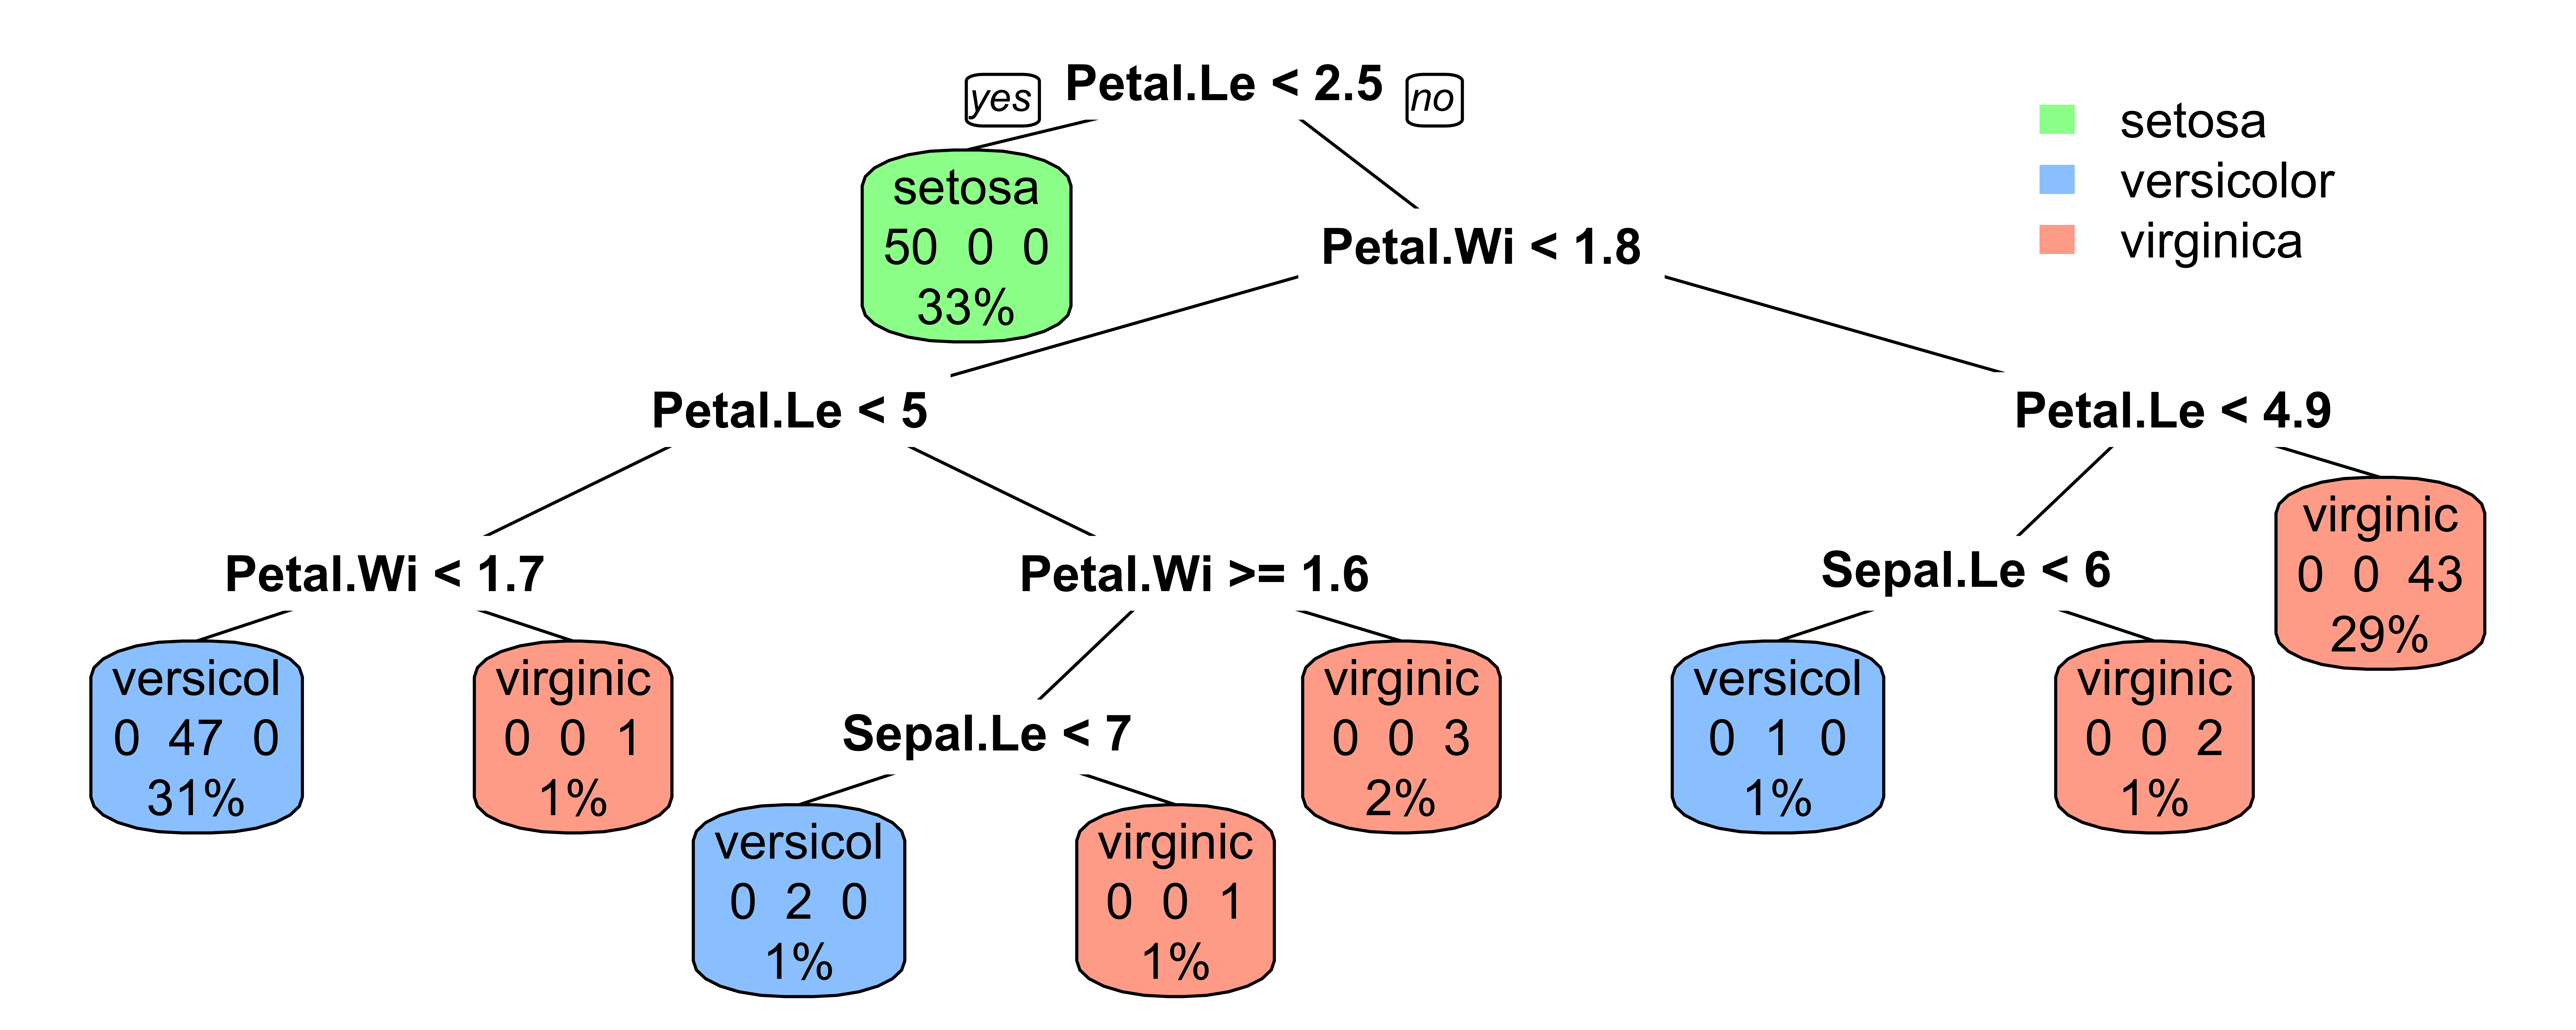
\includegraphics[height=3.5cm]{graphics/plot-rpart.png}
	\vskip 0.1cm 
	{\color{white}AA}
	\includegraphics[height=3.5cm]{graphics/scatter-petalLength-vs-petalWidth-boundaries.png}
	%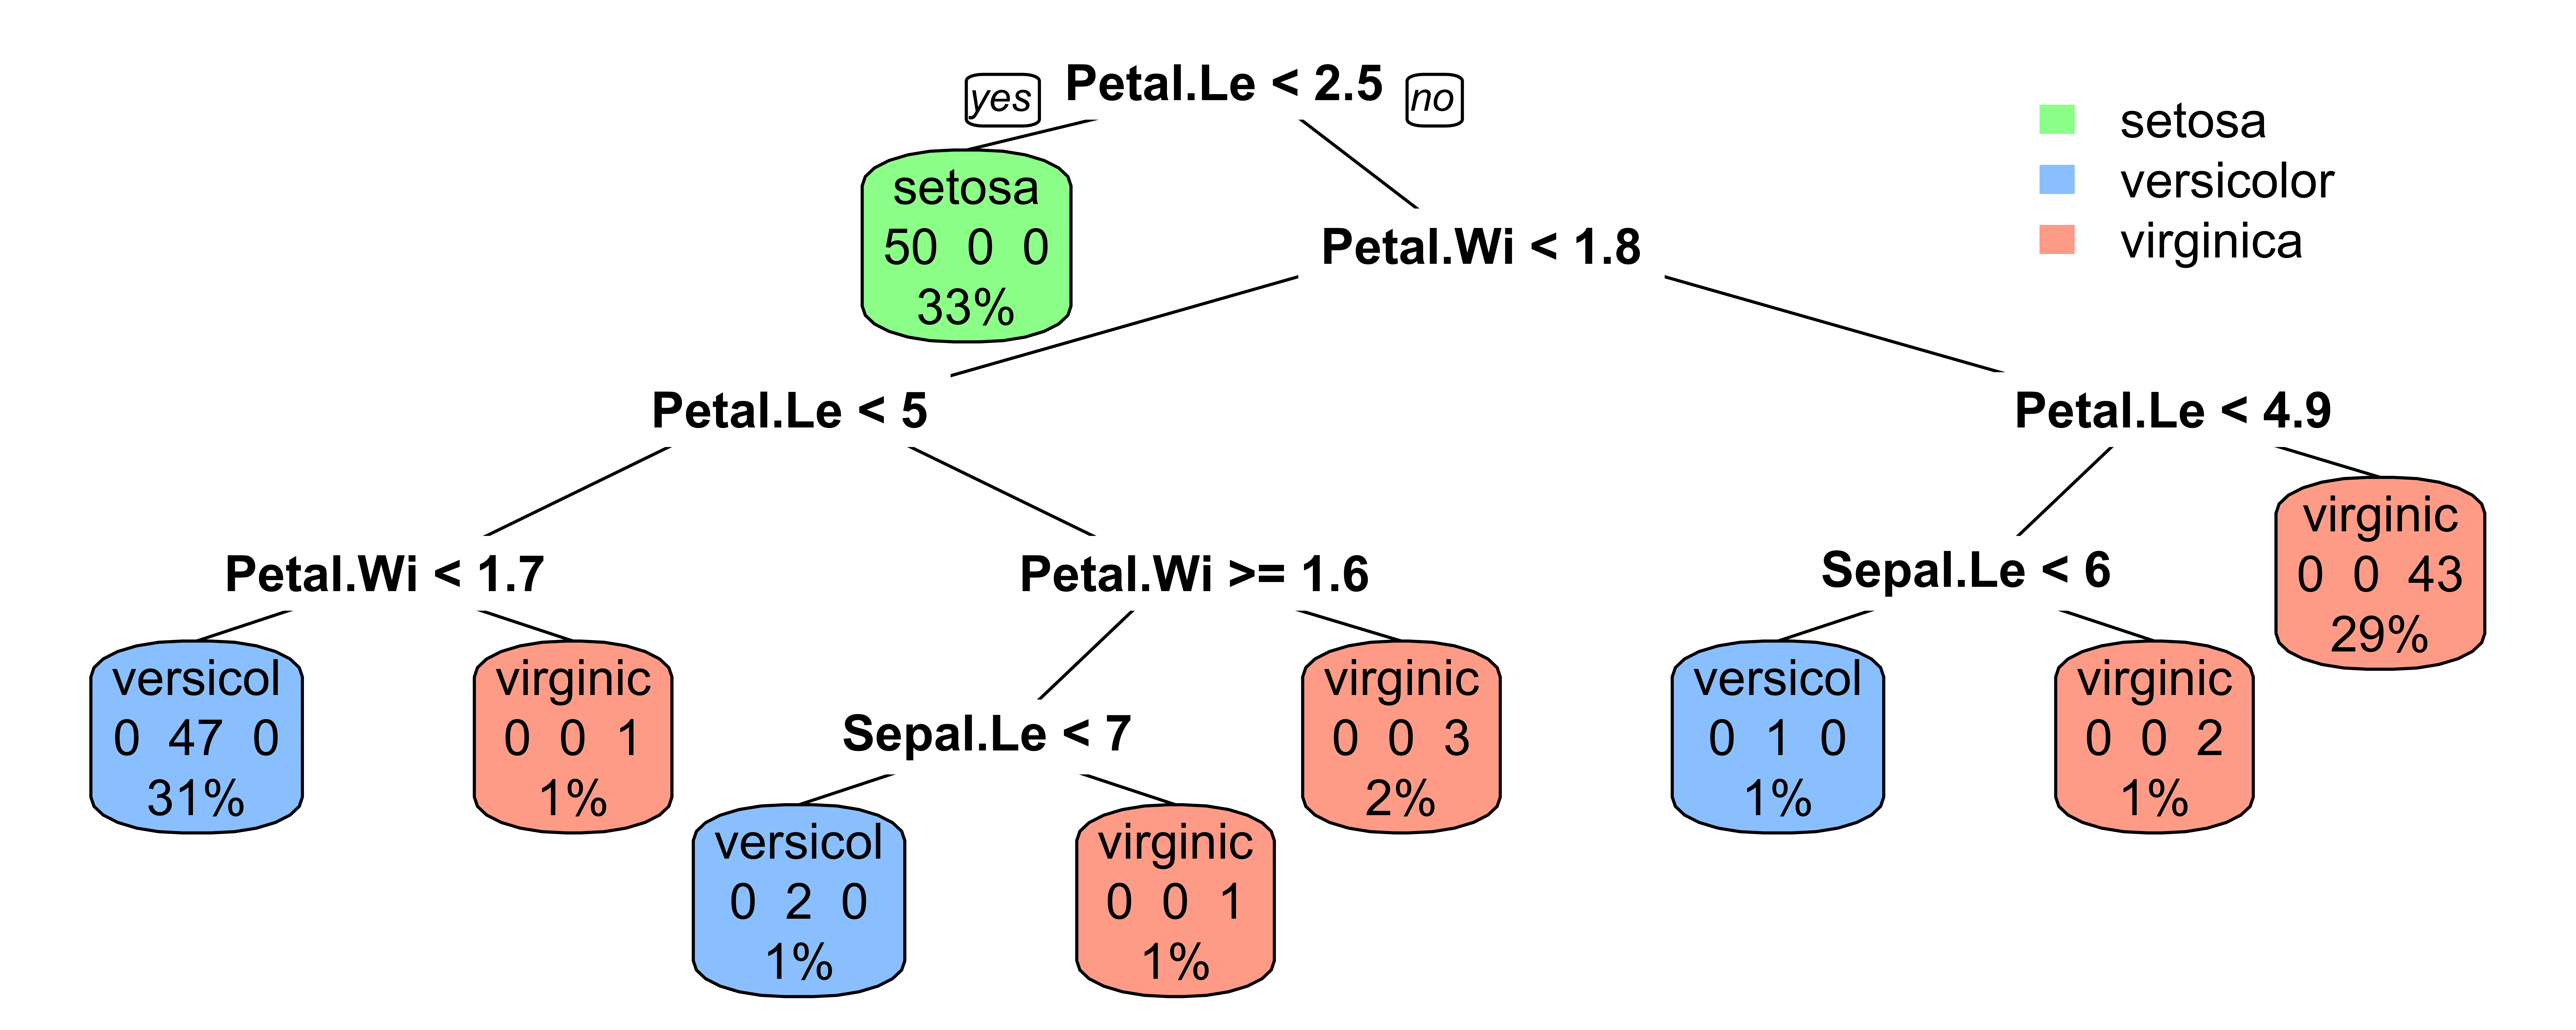
\includegraphics[width=4.5cm,height=6.25cm]{graphics/plot-rpart.png}
	%\includegraphics[width=4.5cm]{graphics/scatter-petalLength-vs-petalWidth-boundaries.png}
	\end{minipage}
	\end{flushright}

\columnbreak

	\begin{flushleft}
	\begin{minipage}{5.75cm}
	%\vskip -0.8cm
	%{\tiny
	%\begin{itemize}
	%\item
	%	\pause
	%	Goal: to find the impurity-minimizing tree.
	%\item
	%	\pause
	%	Hypothesis class is ``essentially'' finite (given data),
	%	but usually too enormous;
	%	\pause
	%	exhaustive search won't work.
	%\end{itemize}}
	\vskip -0.1cm
	\scriptsize
	\pause
	\textbf{\normalsize CART algorithm} (tree-growing step)
	\begin{itemize}
	\item
		\pause
		At each iteration, binary-partition \textbf{\color{red}each} leaf to get the next tree.
	\item
		\pause
		For each leaf, thus need to choose:
		\vskip -0.2cm
		\begin{itemize}
		\setlength{\itemindent}{-0.2in}
		\item
			\pause
			\vskip -0.1cm {\scriptsize``best'' predictor variable to partition by}
		\item
			\pause
			\vskip -0.1cm {\scriptsize``best'' threshold}
		\end{itemize}
	\item
		\pause
		Jensen's inequality \,$\Longrightarrow$\,
		{\color{red}Tree impurity always decreases after partitioning a leaf.}
	\item
		\pause
		For each leaf, choose the (variable,{\color{white}.}threshold)-combo
		that maximizes impurity decrease.
	\item
		\pause
		For each leaf, continue until termination criteria are met.
	%\item
	%	\pause
	%	Computational complexity = $O\!\left(p\,n \log n\right)$
	\end{itemize}
	\end{minipage}
	\end{flushleft}

\end{multicols}

\end{frame}
\normalsize

%%%%%%%%%%

\begin{frame}{\vskip -0.2cm \large The Breiman-Friedman-Olshen-Stone CART Algorithm}

\Large
\textbf{CART Algorithm} (tree-pruning step)

\vskip 0.1cm
\scriptsize
\begin{itemize}
\pause
\item
	For details see:
	\vskip -0.2cm
	{\tiny\begin{itemize}
	\item
		{\tiny Breiman-Friedman-Olshen-Stone, (1984),
		\textit{Classification and Regression Trees}, Taylor \& Francis}
	\item
		\vskip -0.1cm
		{\tiny Ripley, (1996),
		\textit{Pattern Recognition and Neural Networks}, Cambridge University Press}
	\end{itemize}}
\pause
\item
	The tree-growing step tends to produce overfit trees.
\pause
\item
	Grow-then-prune works better than grow-only with strong termination criteria:
	poor-at-first-glance splits may lead to very good splits further down the tree.
\pause
\item
	Once the full tree \,$T_{0}$\, has been grown, use \textbf{cost complexity criterion}
	\vskip -0.1cm
	\begin{equation*}
	C_{{\color{red}\alpha}}(T) \;\; = \;\;
		\#\textnormal{\scriptsize$\left(\!\begin{array}{c}
			\textnormal{misclassified}
			\\
			\textnormal{observations}
		\end{array}\!\right)$}
		\; + \;
		{\color{lightRed}\alpha} \cdot
		\#\textnormal{\scriptsize$\left(\!\begin{array}{c}
			\textnormal{leafs}
			\\
			\textnormal{of $T$}
		\end{array}\!\right)$}
	\end{equation*}
	\vskip -0.1cm
	to assess a given sub-tree $T \subset T_{0}$.
\item
	Fact:
	{\color{red}For each $\alpha \geq 0$,
	\,$T_{\alpha}$ $=$
	$\underset{T \subset T_{0}}{\textnormal{argmin}}\!\left\{\,\overset{{\color{white}.}}{C}_{\alpha}(T)\,\right\}$\,
	exists, is unique, and is computable.}
\item
	To choose optimal $\alpha$, use $5$- or $10$-fold cross-validation:
	Minimize cross-validation misclassification error of $T_{\alpha}$.
\end{itemize}

\end{frame}
\normalsize

%%%%%%%%%%
